\chapter*{Appendix} \label{chap:appendix}


\chapter*{Dodatek} \label{chap:appendix}


\section*{The Fundamental Principles 1889}


\section*{Fundamentalne Zasady 1889}


As elsewhere stated, Seventh-day Adventists have no creed but the Bible; but they hold to certain well-defined points of faith for which they feel prepared to give a reason “to every man that asketh” them. The following propositions may be taken as a summary of the principal features of their religious faith, upon which there is, so far as we know, entire unanimity throughout the body. They believe,—


Jak stwierdzono gdzie indziej, Adwentyści Dnia Siódmego nie mają innego wyznania wiary niż Biblia; ale trzymają się pewnych dobrze zdefiniowanych punktów wiary, dla których czują się przygotowani, aby podać powód “każdemu człowiekowi, który ich pyta”. Poniższe propozycje można uznać za podsumowanie głównych cech ich wiary religijnej, co do których, o ile nam wiadomo, panuje całkowita jednomyślność w całym ciele. Wierzą, że—


\lettrine{I.} That there is one God, a personal, spiritual being, the creator of all things, omnipotent, omniscient, and eternal; infinite in wisdom, holiness, justice, goodness, truth, and mercy; unchangeable, and everywhere present by his representative, the Holy Spirit. Psalm 139:7.


\lettrine{I.} Istnieje jeden Bóg, osobowa, duchowa istota, stwórca wszystkich rzeczy, wszechmocny, wszechwiedzący i wieczny; nieskończony w mądrości, świętości, sprawiedliwości, dobroci, prawdzie i miłosierdziu; niezmienny i wszędzie obecny przez swojego przedstawiciela, Ducha Świętego. Psalm 139:7.


\lettrine{II.} That there is one Lord Jesus Christ, the Son of the Eternal Father, the one by whom he created all things, and by whom they do consist; that he took on him the nature of the seed of Abraham for the redemption of our fallen race; that he dwelt among men, full of grace and truth, lived our example, died our sacrifice, was raised for our justification, ascended on high to be our only mediator in the sanctuary in heaven, where, through the merits of his shed blood, he secures the pardon and forgiveness of the sins of all those who penitently come to him; and as the closing portion of his work as priest, before he takes his throne as king, he will make the great atonement for the sins of all such, and their sins will then be blotted out (Acts 3:19) and borne away from the sanctuary, as shown in the service of the Levitical priesthood, which foreshadowed and prefigured the ministry of our Lord in heaven. See Leviticus 16; Hebrews 8:4, 5; 9:6, 7; etc.


\lettrine{II.} Istnieje jeden Pan Jezus Chrystus, Syn Wiecznego Ojca, ten, przez którego stworzył wszystkie rzeczy i przez którego one istnieją; że przyjął On naturę nasienia Abrahama dla odkupienia naszej upadłej rasy; że mieszkał wśród ludzi, pełen łaski i prawdy, żył jako nasz przykład, umarł jako nasza ofiara, został wskrzeszony dla naszego usprawiedliwienia, wstąpił na wysokości, aby być naszym jedynym pośrednikiem w świątyni w niebie, gdzie przez zasługi swojej przelanej krwi zapewnia przebaczenie i odpuszczenie grzechów wszystkim tym, którzy skruszeni przychodzą do Niego; i jako końcowa część Jego dzieła jako kapłana, zanim obejmie swój tron jako król, dokona wielkiego pojednania za grzechy wszystkich takich, a ich grzechy zostaną wtedy wymazane (Dzieje 3:19) i usunięte ze świątyni, jak pokazano w służbie kapłaństwa lewickiego, które zapowiadało i prefigurowało posługę naszego Pana w niebie. Zobacz Kapłańska 16; Hebrajczyków 8:4, 5; 9:6, 7; itd.


\lettrine{III.} That the Holy Scriptures of the Old and New Testaments were given by inspiration of God, contain a full revelation of his will to man, and are the only infallible rule of faith and practice.


\lettrine{III.} Że Święte Pisma Starego i Nowego Testamentu zostały dane przez natchnienie Boże, zawierają pełne objawienie Jego woli wobec człowieka i są jedyną nieomylną regułą wiary i praktyki.


\lettrine{IV.} That baptism is an ordinance of the Christian church, to follow faith and repentance,—an ordinance by which we commemorate the resurrection of Christ, as by this act we show our faith in his burial and resurrection, and through that, in the resurrection of all the saints at the last day; and that no other mode more fitly represents these facts than that which the Scriptures prescribe, namely, immersion. Romans 6:3-5; Colossians 2:12.


\lettrine{IV.} Że chrzest jest obrzędem kościoła chrześcijańskiego, następującym po wierze i pokucie — obrzędem, przez który upamiętniamy zmartwychwstanie Chrystusa, ponieważ przez ten akt pokazujemy naszą wiarę w Jego pogrzeb i zmartwychwstanie, a przez to w zmartwychwstanie wszystkich świętych w dniu ostatecznym; i że żaden inny sposób nie przedstawia tych faktów lepiej niż ten, który przepisuje Pismo Święte, a mianowicie zanurzenie. Rzymian 6:3-5; Kolosan 2:12.


\lettrine{V.} That the new birth comprises the entire change necessary to fit us for the kingdom of God, and consists of two parts; First, a moral change wrought by conversion and a Christian life (John 3:3, 5); second, a physical change at the second coming of Christ, whereby, if dead, we are raised incorruptible, and if living, are changed to immortality in a moment, in the twinkling of an eye. Luke 20:36; 1 Corinthians 15:51, 52.


\lettrine{V.} Że nowe narodzenie obejmuje całą zmianę niezbędną do przygotowania nas do królestwa Bożego i składa się z dwóch części; Po pierwsze, zmiana moralna dokonana przez nawrócenie i chrześcijańskie życie (Jan 3:3, 5); po drugie, zmiana fizyczna przy powtórnym przyjściu Chrystusa, przez którą, jeśli umarliśmy, zostaniemy wskrzeszeni jako niezniszczalni, a jeśli żyjemy, zostaniemy przemienieni w nieśmiertelność w jednej chwili, w mgnieniu oka. Łukasz 20:36; 1 Koryntian 15:51, 52.


\lettrine{VI.} That prophecy is a part of God’s revelation to man; that it is included in that Scripture which is profitable for instruction (2 Timothy 3:16); that it is designed for us and our children (Deuteronomy 29:29); that so far from being enshrouded in impenetrable mystery, it is that which especially constitutes the word of God a lamp to our feet and a light to our path (Psalm 119:105; 2 Peter 1:19); that a blessing is pronounced upon those who study it (Revelation 1:1-3); and that, consequently, it is to be understood by the people of God sufficiently to show them their position in the world’s history and the special duties required at their hands.


\lettrine{VI.} Że proroctwo jest częścią Bożego objawienia dla człowieka; że jest zawarte w tym Piśmie, które jest pożyteczne do nauki (2 Tymoteusza 3:16); że jest przeznaczone dla nas i naszych dzieci (Powtórzonego Prawa 29:29); że dalekie od bycia spowite w nieprzeniknioną tajemnicę, jest tym, co szczególnie stanowi słowo Boże jako lampę dla naszych stóp i światło na naszej ścieżce (Psalm 119:105; 2 Piotra 1:19); że błogosławieństwo jest ogłoszone nad tymi, którzy je studiują (Objawienie 1:1-3); i że w konsekwencji ma być zrozumiane przez lud Boży w stopniu wystarczającym, aby pokazać im ich pozycję w historii świata i szczególne obowiązki wymagane z ich rąk.


\lettrine{VII.} That the world’s history from specified dates in the past, the rise and fall of empires, and the chronological succession of events down to the setting up of God’s everlasting kingdom, are outlined in numerous great chains of prophecy; and that these prophecies are now all fulfilled except the closing scenes.


\lettrine{VII.} Że historia świata od określonych dat w przeszłości, wzrost i upadek imperiów oraz chronologiczna sukcesja wydarzeń aż do ustanowienia wiecznego królestwa Bożego, są zarysowane w licznych wielkich łańcuchach proroctw; i że te proroctwa są teraz wszystkie wypełnione z wyjątkiem końcowych scen.


\lettrine{VIII.} That the doctrine of the world’s conversion and a temporal millennium is a fable of these last days, calculated to lull men into a state of carnal security, and cause them to be overtaken by the great day of the Lord as by a thief in the night (1 Thessalonians 5:3); that the second coming of Christ is to precede, not follow, the millennium; for until the Lord appears, the papal power, with all its abominations, is to continue (2 Thessalonians 2:8), the wheat and tares grow together (Matthew 13:29, 30, 39), and evil men and seducers wax worse and worse, as the word of God declares. 2 Timothy 3:1, 13.


\lettrine{VIII.} Że doktryna o nawróceniu świata i doczesnym tysiącleciu jest bajką tych ostatnich dni, obliczoną na uśpienie ludzi w stan cielesnego bezpieczeństwa i spowodowanie, że wielki dzień Pański zaskoczy ich jak złodziej w nocy (1 Tesaloniczan 5:3); że drugie przyjście Chrystusa ma poprzedzać, a nie następować po tysiącleciu; ponieważ dopóki Pan się nie pojawi, papieska władza, ze wszystkimi swoimi obrzydliwościami, będzie trwać (2 Tesaloniczan 2:8), pszenica i kąkol będą rosnąć razem (Mateusz 13:29, 30, 39), a źli ludzie i zwodziciele będą stawać się coraz gorsi, jak głosi Słowo Boże. 2 Tymoteusza 3:1, 13.


\lettrine{IX.} That the mistake of Adventists in 1844 pertained to the nature of the event then to transpire, not to the time; that no prophetic period is given to reach to the second advent, but that the longest one, the two thousand and three hundred days of Daniel 8:14, terminated in 1844, and brought us to an event called the cleansing of the sanctuary.


\lettrine{IX.} Że pomyłka Adwentystów w 1844 roku dotyczyła natury wydarzenia, które miało wówczas nastąpić, a nie czasu; że żaden okres proroczy nie jest dany, aby sięgał do drugiego przyjścia, ale że najdłuższy z nich, dwa tysiące trzysta dni z Daniela 8:14, zakończył się w 1844 roku i doprowadził nas do wydarzenia zwanego oczyszczeniem świątyni.


\lettrine{X.} That the sanctuary of the new covenant is the tabernacle of God in heaven, of which Paul speaks in Hebrews 8 and onward, and of which our Lord, as great high priest, is minister; that this sanctuary is the antitype of the Mosaic tabernacle, and that the priestly work of our Lord, connected therewith, is the antitype of the work of the Jewish priests of the former dispensation (Hebrews 8:1-5, etc.); that this, and not the earth, is the sanctuary to be cleansed at the end of the two thousand and three hundred days, what is termed its cleansing being in this case, as in the type, simply the entrance of the high priest into the most holy place, to finish the round of service connected therewith, by making the atonement and removing from the sanctuary the sins which had been transferred to it by means of the ministration in the first apartment (Leviticus 16; Hebrews 9:22, 23); and that this work in the antitype, beginning in 1844, consists in actually blotting out the sins of believers (Acts 3:19), and occupies a brief but indefinite space of time, at the conclusion of which the work of mercy for the world will be finished, and the second advent of Christ will take place.


\lettrine{X.} Że świątynia nowego przymierza to przybytek Boży w niebie, o którym Paweł mówi w Liście do Hebrajczyków 8 i dalej, a którego nasz Pan, jako wielki arcykapłan, jest sługą; że ta świątynia jest antytypem przybytku Mojżeszowego, a kapłańska praca naszego Pana, z nią związana, jest antytypem pracy żydowskich kapłanów poprzedniego porządku (Hebrajczyków 8:1-5, itd.); że to, a nie ziemia, jest świątynią, która ma być oczyszczona na końcu dwóch tysięcy trzystu dni, a to, co nazywa się jej oczyszczeniem, jest w tym przypadku, jak w typie, po prostu wejściem arcykapłana do miejsca najświętszego, aby zakończyć cykl służby z tym związanej, dokonując pojednania i usuwając ze świątyni grzechy, które zostały do niej przeniesione za pomocą posługi w pierwszym przedziale (Kapłańska 16; Hebrajczyków 9:22, 23); i że ta praca w antytypie, rozpoczynająca się w 1844 roku, polega na faktycznym wymazywaniu grzechów wierzących (Dzieje Apostolskie 3:19) i zajmuje krótki, ale nieokreślony czas, po zakończeniu którego dzieło miłosierdzia dla świata zostanie zakończone, a drugie przyjście Chrystusa nastąpi.


\lettrine{XI.} That God’s moral requirements are the same upon all men in all dispensations; that these are summarily contained in the commandments spoken by Jehovah from Sinai, engraven on the tables of stone, and deposited in the ark, which was in consequence called the “ark of the covenant,” or testament (Numbers 10:33; Hebrews 9:4, etc.); that this law is immutable and perpetual, being a transcript of the tables deposited in the ark in the true sanctuary on high, which is also, for the same reason, called the ark of God’s testament; for under the sounding of the seventh trumpet we are told that “the temple of God was opened in heaven, and there was seen in his temple the ark of his testament.” Revelation 11:19.


\lettrine{XI.} Że moralne wymagania Boga są takie same dla wszystkich ludzi we wszystkich porządkach; że są one zawarte w przykazaniach wypowiedzianych przez Jehowę z Synaju, wyrytych na kamiennych tablicach i złożonych w arce, która w konsekwencji została nazwana “arką przymierza” lub testamentu (Liczb 10:33; Hebrajczyków 9:4, itd.); że to prawo jest niezmienne i wieczne, będąc odpisem tablic złożonych w arce w prawdziwej świątyni w górze, która również, z tego samego powodu, nazywana jest arką testamentu Bożego; ponieważ przy dźwięku siódmej trąby powiedziano nam, że “świątynia Boża w niebie została otwarta i widziano w Jego świątyni arkę Jego testamentu”. Objawienie 11:19.


\lettrine{XII.} That the fourth commandment of this law requires that we devote the seventh day of each week, commonly called Saturday, to abstinence from our own labor, and to the performance of sacred and religious duties; that this is the only weekly Sabbath known to the Bible, being the day that was set apart before Paradise was lost (Genesis 2:2, 3), and which will be observed in Paradise restored (Isaiah 66:22, 23); that the facts upon which the Sabbath institution is based confine it to the seventh day, as they are not true of any other day; and that the terms Jewish Sabbath, as applied to the seventh day, and Christian Sabbath, as applied to the first day of the week, are names of human invention, unscriptural in fact, and false in meaning.


\lettrine{XII.} Że czwarte przykazanie tego prawa wymaga, abyśmy poświęcili siódmy dzień każdego tygodnia, powszechnie zwany sobotą, na powstrzymanie się od własnej pracy i na wykonywanie świętych i religijnych obowiązków; że jest to jedyny cotygodniowy szabat znany Biblii, będący dniem, który został oddzielony zanim raj został utracony (Rodzaju 2:2, 3) i który będzie przestrzegany w przywróconym raju (Izajasza 66:22, 23); że fakty, na których opiera się instytucja szabatu, ograniczają go do siódmego dnia, ponieważ nie są one prawdziwe dla żadnego innego dnia; i że terminy żydowski szabat, stosowany do siódmego dnia, i chrześcijański szabat, stosowany do pierwszego dnia tygodnia, są nazwami ludzkiego wynalazku, niebiblijne w fakcie i fałszywe w znaczeniu.


\lettrine{XIII.} That as the man of sin, the papacy, has thought to change times and laws (the law of God, Daniel 7:25), and has misled almost all Christendom in regard to the fourth commandment, we find a prophecy of a reform in this respect to be wrought among believers just before the coming of Christ. Isaiah 56:1, 2; 1 Peter 1:5; Revelation 14:12, etc.


\lettrine{XIII.} Że ponieważ człowiek grzechu, papiestwo, zamierzał zmienić czasy i prawa (prawo Boże, Daniela 7:25) i wprowadził w błąd prawie całe chrześcijaństwo w odniesieniu do czwartego przykazania, znajdujemy proroctwo o reformie w tym względzie, która ma być dokonana wśród wierzących tuż przed przyjściem Chrystusa. Izajasza 56:1, 2; 1 Piotra 1:5; Objawienie 14:12, itd.


\lettrine{XIV.} That the followers of Christ should be a peculiar people, not following the maxims, nor conforming to the ways, of the world; not loving its pleasures nor countenancing its follies; inasmuch as the apostle says that “whosoever therefore will be” in this sense, “a friend of the world, is the enemy of God” (James 4:4); and Christ says that we cannot have two masters, or, at the same time, serve God and mammon. Matthew 6:24.


\lettrine{XIV.} Że naśladowcy Chrystusa powinni być szczególnym ludem, nie podążającym za maksymami ani nie dostosowującym się do dróg świata; nie kochającym jego przyjemności ani nie pobłażającym jego głupocie; o tyle, o ile apostoł mówi, że “ktokolwiek więc chce być” w tym sensie “przyjacielem świata, staje się wrogiem Boga” (Jakuba 4:4); a Chrystus mówi, że nie możemy mieć dwóch panów ani jednocześnie służyć Bogu i mamonie. Mateusza 6:24.


\lettrine{XV.} That the Scriptures insist upon plainness and modesty of attire as a prominent mark of discipleship in those who profess to be the followers of Him who was, “meek and lowly in heart,” that the wearing of gold, pearls, and costly array, or anything designed merely to adorn the person and foster the pride of the natural heart, is to be discarded, according to such scriptures as 1 Timothy 2:9, 10; 1 Peter 3:3, 4.


\lettrine{XV.} Że Pisma kładą nacisk na prostotę i skromność stroju jako wyraźny znak uczniostwa u tych, którzy twierdzą, że są naśladowcami Tego, który był “cichy i pokornego serca”, że noszenie złota, pereł i kosztownych strojów, lub czegokolwiek przeznaczonego jedynie do ozdoby osoby i podsycania dumy naturalnego serca, należy odrzucić, zgodnie z takimi fragmentami Pisma jak 1 Tymoteusza 2:9, 10; 1 Piotra 3:3, 4.


\lettrine{XVI.} That means for the support of evangelical work among men should be contributed from love to God and love of souls, not raised by church lotteries, or occasions designed to contribute to the fun-loving, appetite-indulging propensities of the sinner, such as fairs, festivals, oyster suppers, tea, broom, donkey, and crazy socials, etc., which are a disgrace to the professed church of Christ; that the proportion of one’s income required in former dispensation can be no less under the gospel; that it is the same as Abraham (whose children we are, if we are Christ’s, Galatians 3:29) paid to Melchisedec (type of Christ) when he gave him a tenth of all (Hebrews 7:1-4); the title is the Lord’s (Leviticus 27:30); and this tenth of one’s income is also to be supplemented by offerings from those who are able, for the support of the gospel. 2 Corinthians 9:6; Malachi 3:8, 10.


\lettrine{XVI.} Że środki na wsparcie pracy ewangelicznej wśród ludzi powinny być przekazywane z miłości do Boga i miłości do dusz, a nie pozyskiwane przez loterie kościelne lub okazje mające przyczyniać się do miłujących zabawę, dogadzających apetytowi skłonności grzesznika, takie jak targi, festiwale, kolacje ostrygowe, herbatki, miotły, osły i szalone spotkania towarzyskie itp., które są hańbą dla wyznającego kościoła Chrystusa; że proporcja dochodu wymagana w poprzednich porządkach nie może być mniejsza pod ewangelią; że jest taka sama, jaką Abraham (którego dziećmi jesteśmy, jeśli należymy do Chrystusa, Galacjan 3:29) zapłacił Melchizedekowi (typowi Chrystusa), gdy dał mu dziesiątą część wszystkiego (Hebrajczyków 7:1-4); dziesięcina należy do Pana (Kapłańska 27:30); i ta dziesiąta część dochodu ma być również uzupełniona ofiarami od tych, którzy są w stanie, na wsparcie ewangelii. 2 Koryntian 9:6; Malachiasza 3:8, 10.


\lettrine{XVII.} That as the natural or carnal heart is at enmity with God and his law, this enmity can be subdued only by a radical transformation of the affections, the exchange of unholy for holy principles; that this transformation follows repentance and faith, is the special work of the Holy Spirit, and constitutes regeneration, or conversion.


\lettrine{XVII.} Że ponieważ naturalne lub cielesne serce jest wrogie Bogu i Jego prawu, ta wrogość może być poskromiona tylko przez radykalną transformację uczuć, wymianę nieczystych zasad na święte; że ta transformacja następuje po pokucie i wierze, jest szczególnym dziełem Ducha Świętego i stanowi odrodzenie lub nawrócenie.


\lettrine{XVIII.} That as all have violated the law of God, and cannot of themselves render obedience to his just requirements, we are dependent on Christ, first, for justification from our past offenses, and, secondly, for grace whereby to render acceptable obedience to his holy law in time to come.


\lettrine{XVIII.} Ponieważ wszyscy naruszyli prawo Boże i nie mogą sami z siebie okazać posłuszeństwa Jego sprawiedliwym wymaganiom, jesteśmy zależni od Chrystusa, po pierwsze, dla usprawiedliwienia z naszych przeszłych wykroczeń, a po drugie, dla łaski, dzięki której możemy okazać akceptowalne posłuszeństwo Jego świętemu prawu w przyszłości.


\lettrine{XIX.} That the Spirit of God was promised to manifest itself in the church through certain gifts, enumerated especially in 1 Corinthians 12 and Ephesians 4; that these gifts are not designed to supersede, or take the place of, the Bible, which is sufficient to make us wise unto salvation, any more than the Bible can take the place of the Holy Spirit; that, in specifying the various channels of its operation, that Spirit has simply made provision for its own existence and presence with the people of God to the end of time, to lead to an understanding of that word which it had inspired, to convince of sin, and to work a transformation in the heart and life; and that those who deny to the Spirit its place and operation, do plainly deny that part of the Bible which assigns to it this work and position.


\lettrine{XIX.} Że Duch Boży został obiecany, aby objawić się w kościele poprzez pewne dary, wymienione szczególnie w 1 Koryntian 12 i Efezjan 4; że te dary nie są przeznaczone do zastąpienia lub zajęcia miejsca Biblii, która jest wystarczająca, aby uczynić nas mądrymi ku zbawieniu, tak jak Biblia nie może zająć miejsca Ducha Świętego; że określając różne kanały swojego działania, ten Duch po prostu zapewnił swoje własne istnienie i obecność z ludem Bożym aż do końca czasu, aby prowadzić do zrozumienia tego słowa, które natchnął, aby przekonać o grzechu i dokonać przemiany w sercu i życiu; i że ci, którzy odmawiają Duchowi jego miejsca i działania, wyraźnie zaprzeczają tej części Biblii, która przypisuje mu to dzieło i pozycję.


\lettrine{XX.} That God, in accordance with his uniform dealings with the race, sends forth a proclamation of the approach of the second advent of Christ; and that this work is symbolized by the three messages of Revelation 14, the last one bringing to view the work of reform on the law of God, that his people may acquire a complete readiness for that event.


\lettrine{XX.} Że Bóg, zgodnie ze swoim jednolitym postępowaniem wobec rasy ludzkiej, ogłasza proklamację o zbliżaniu się drugiego przyjścia Chrystusa; i że ta praca jest symbolizowana przez trzy poselstwa z Objawienia 14, z których ostatnie ukazuje dzieło reformy prawa Bożego, aby Jego lud mógł osiągnąć pełną gotowość na to wydarzenie.


\lettrine{XXI.} That the time of the cleansing of the sanctuary (See proposition X.), synchronizing with the time of the proclamation of the third message (Revelation 14:9, 10), is a time of investigative judgment, first, with reference to the dead, and secondly, at the close of probation, with reference to the living, to determine who of the myriads now sleeping in the dust of the earth are worthy of a part in the first resurrection, and who of its living multitudes are worthy of translation,—points which must be determined before the Lord appears.


\lettrine{XXI.} Że czas oczyszczenia świątyni (Patrz propozycja X.), synchronizujący się z czasem głoszenia trzeciego poselstwa (Objawienie 14:9, 10), jest czasem sądu śledczego, po pierwsze, w odniesieniu do zmarłych, a po drugie, przy końcu czasu próby, w odniesieniu do żyjących, aby określić, którzy z niezliczonych obecnie śpiących w prochu ziemi są godni udziału w pierwszym zmartwychwstaniu, i którzy z żyjących tłumów są godni przemienienia – punkty, które muszą być określone zanim Pan się pojawi.


\lettrine{XXII.} That the grave, whether we all tend, expressed by the Hebrew word sheol and the Greek word hades, is a place, or condition, in which there is no work, device, wisdom, nor knowledge. Ecclesiastes 9:10.


\lettrine{XXII.} Że grób, do którego wszyscy zmierzamy, wyrażony hebrajskim słowem sheol i greckim słowem hades, jest miejscem lub stanem, w którym nie ma pracy, zamysłu, mądrości ani wiedzy. Księga Kaznodziei 9:10.


\lettrine{XXIII.} That the state to which we are reduced by death is one of silence, inactivity, and entire unconsciousness. Psalm 146:4; Ecclesiastes 9:5, 6; Daniel 12:2.


\lettrine{XXIII.} Że stan, do którego jesteśmy zredukowani przez śmierć, jest stanem ciszy, bezczynności i całkowitej nieświadomości. Psalm 146:4; Księga Kaznodziei 9:5, 6; Daniela 12:2.


\lettrine{XXIV.} That out of this prison-house of the grave, mankind are to be brought by a bodily resurrection; the righteous having part in the first resurrection, which takes place at the second coming of Christ; the wicked, in the second resurrection, which takes place in a thousand years thereafter. Revelation 20:4-6.


\lettrine{XXIV.} Że z tego więzienia grobu ludzkość zostanie wyprowadzona przez cielesne zmartwychwstanie; sprawiedliwi mają udział w pierwszym zmartwychwstaniu, które następuje przy drugim przyjściu Chrystusa; bezbożni, w drugim zmartwychwstaniu, które następuje tysiąc lat później. Objawienie 20:4-6.


\lettrine{XXV.} That at the last trump, the living righteous are to be changed in a moment, in the twinkling of an eye, and with the risen righteous are to be caught up to meet the Lord in the air, so forever to be with the Lord. 1 Thessalonians 4:16, 17; 1 Corinthians 15:51, 52.


\lettrine{XXV.} Że przy ostatniej trąbie żyjący sprawiedliwi zostaną przemienieni w jednej chwili, w mgnieniu oka, i wraz ze zmartwychwstałymi sprawiedliwymi zostaną porwani, aby spotkać Pana w powietrzu, aby na zawsze być z Panem. 1 Tesaloniczan 4:16, 17; 1 Koryntian 15:51, 52.


\lettrine{XXVI.} That these immortalized ones are then taken to heaven, to the New Jerusalem, the Father’s house, in which there are many mansions (John 14:1-3), where they reign with Christ a thousand years, judging the world and fallen angels, that is, apportioning the punishment to be executed upon them at the close of the one thousand years (Revelation 20:4; 1 Corinthians 6:2, 3); that during this time the earth lies in a desolate and chaotic condition (Jeremiah 4:23-27), described, as in the beginning, by the Greek term abussos— “bottom-less pit” (Septuagint of Genesis 1:2); and that here Satan is confined during the thousand years (Revelation 20:1, 2), and here finally destroyed (Revelation 20:10; Malachi 4:1); the theater of the ruin he has wrought in the universe being appropriately made, for a time, his gloomy prison-house, and then the place of his final execution.


\lettrine{XXVI.} Że ci nieśmiertelni są następnie zabrani do nieba, do Nowego Jeruzalem, domu Ojca, w którym jest wiele mieszkań (Jana 14:1-3), gdzie królują z Chrystusem przez tysiąc lat, sądząc świat i upadłych aniołów, to znaczy wyznaczając karę, która ma być wykonana na nich pod koniec tysiąca lat (Objawienie 20:4; 1 Koryntian 6:2, 3); że w tym czasie ziemia leży w stanie spustoszenia i chaosu (Jeremiasza 4:23-27), opisanym, jak na początku, greckim terminem abussos – “bezdenną otchłanią” (Septuaginta z Księgi Rodzaju 1:2); i że tutaj Szatan jest uwięziony przez tysiąc lat (Objawienie 20:1, 2), i tutaj ostatecznie zniszczony (Objawienie 20:10; Malachiasza 4:1); teatr zniszczenia, którego dokonał we wszechświecie, staje się odpowiednio, na pewien czas, jego ponurym więzieniem, a następnie miejscem jego ostatecznej egzekucji.


\lettrine{XXVII.} That at the end of the thousand years the Lord descends with his people and the New Jerusalem (Revelation 21:2), the wicked dead are raised, and come up on the surface of the yet unrenewed earth, and gather about the city, the camp of the saints (Revelation 20:9), and fire comes down from God out of heaven and devours them. They are then consumed, root and branch (Malachi 4:1), becoming as though they had not been. Obadiah 15, 16. In this everlasting destruction from the presence of the Lord (2 Thessalonians 1:9), the wicked meet the “everlasting punishment” threatened against them (Matthew 25:46), which is everlasting death. Romans 6:23; Revelation 20:14, 15. This is the perdition of ungodly men, the fire which consumes them being the fire for which “the heavens and the earth, which are now,... are kept in store.” which shall melt even the elements with its intensity, and purge the earth from the deepest stains of the curse of sin. 2 Peter 3:7-12.


\lettrine{XXVII.} Że pod koniec tysiąca lat Pan zstępuje ze swoim ludem i Nowym Jeruzalem (Objawienie 21:2), bezbożni zmarli są wskrzeszeni i wychodzą na powierzchnię jeszcze nieodnowionej ziemi, i gromadzą się wokół miasta, obozu świętych (Objawienie 20:9), a ogień zstępuje od Boga z nieba i pożera ich. Są wtedy strawieni, korzeń i gałąź (Malachiasza 4:1), stając się, jakby ich nie było. Abdiasza 15, 16. W tym wiecznym zniszczeniu od obecności Pana (2 Tesaloniczan 1:9), bezbożni spotykają “wieczną karę” im zagrożoną (Mateusza 25:46), która jest wieczną śmiercią. Rzymian 6:23; Objawienie 20:14, 15. To jest zatracenie bezbożnych ludzi, ogień, który ich pochłania, będąc ogniem, dla którego “niebiosa i ziemia, które są teraz,... są zachowane”, który stopi nawet żywioły swoją intensywnością i oczyści ziemię z najgłębszych plam przekleństwa grzechu. 2 Piotra 3:7-12.


\lettrine{XXVIII.} That new heavens and a new earth shall spring by the power of God from the ashes of the old, and this renewed earth, with the New Jerusalem for its metropolis and capital, shall be the eternal inheritance of the saints, the place where the righteous shall evermore dwell. 2 Peter 3:13; Psalm 37:11, 29; Matthew 5:5.


\lettrine{XXVIII.} Że nowe niebo i nowa ziemia powstaną mocą Bożą z popiołów starego, a ta odnowiona ziemia, z Nowym Jeruzalem jako jej metropolią i stolicą, będzie wiecznym dziedzictwem świętych, miejscem, gdzie sprawiedliwi będą mieszkać na wieki. 2 Piotra 3:13; Psalm 37:11, 29; Mateusza 5:5.


\section*{Fundamental Principles - Timeline} \label{appendix:timeline}


\section*{Fundamentalne Zasady - Oś czasu} \label{appendix:timeline}


The following is a list of some appearances of the Declaration of Fundamental Principles in our publications. All links are accessible at \href{https://notefp.link/fp-timeline}{https://notefp.link/fp-timeline}.


Poniżej znajduje się lista niektórych wystąpień Oświadczenia o fundamentalnych zasadach w naszych publikacjach. Wszystkie linki są dostępne na \href{https://notefp.link/fp-timeline}{https://notefp.link/fp-timeline}.


\leftsubsection{1872 - The first appearance}


\leftsubsection{1872 - Pierwsze pojawienie się}


\textit{“A Declaration of the Fundamental Principles Taught and Practiced by Seventh-day Adventists}” - printed as a pamphlet (\href{https://adventistdigitallibrary.org/islandora/object/adl:366607?link_only=true}{original scan} \href{https://forgotten-pillar.s3.us-east-2.amazonaws.com/A+declaration+of+the+fundamental+principles+taught+and+practiced+by+the+Seventh-day+Adventists++.pdf}{*}). They appeared anonymous, presented as a short public synopsis of what Seventh-day Adventists believe.


\textit{“Oświadczenie o fundamentalnych zasadach nauczanych i wyznawanych przez Adwentystów Dnia Siódmego”} - wydrukowane jako broszura (\href{https://adventistdigitallibrary.org/islandora/object/adl:366607?link_only=true}{oryginalny skan} \href{https://forgotten-pillar.s3.us-east-2.amazonaws.com/A+declaration+of+the+fundamental+principles+taught+and+practiced+by+the+Seventh-day+Adventists++.pdf}{*}). Pojawiły się anonimowo, przedstawione jako krótkie publiczne streszczenie tego, w co wierzą Adwentyści Dnia Siódmego.


\leftsubsection{1874 - The Signs of the Times}


\leftsubsection{1874 - The Signs of the Times}


Original scan: \href{https://adventistdigitallibrary.org/adl-364148/signs-times-june-4-1874}{ST June 4, 1874, p.3.} \href{https://forgotten-pillar.s3.us-east-2.amazonaws.com/Signs+of+the+Times+_+June+4%2C+1874++.pdf}{*} James White stood behind the declaration as a main editor of the Signs of the Times at that time.


Oryginalny skan: \href{https://adventistdigitallibrary.org/adl-364148/signs-times-june-4-1874}{ST 4 czerwca 1874, s.3.} \href{https://forgotten-pillar.s3.us-east-2.amazonaws.com/Signs+of+the+Times+_+June+4%2C+1874++.pdf}{*} James White stał za oświadczeniem jako główny redaktor Signs of the Times w tym czasie.


\leftsubsection{1874 - The Advent Review and Herald of the Sabbath}


\leftsubsection{1874 - The Advent Review and Herald of the Sabbath}


Original scan: \href{https://documents.adventistarchives.org/Periodicals/RH/RH18741124-V44-22.pdf}{RH November 24, 1874, p.171} \href{https://forgotten-pillar.s3.us-east-2.amazonaws.com/RH18741124-V44-22.pdf}{*} Uriah Smith signed the declaration as the main editor of the Review and Herald of the Sabbath periodical at that time.


Oryginalny skan: \href{https://documents.adventistarchives.org/Periodicals/RH/RH18741124-V44-22.pdf}{RH 24 listopada 1874, s.171} \href{https://forgotten-pillar.s3.us-east-2.amazonaws.com/RH18741124-V44-22.pdf}{*} Uriah Smith podpisał oświadczenie jako główny redaktor periodyka Review and Herald of the Sabbath w tym czasie.


\leftsubsection{1874 - Part of a booklet: The Seventh-day Adventists: A Brief Sketch of Their Origin, Progress, and Principles}


\leftsubsection{1874 - Część broszury: The Seventh-day Adventists: A Brief Sketch of Their Origin, Progress, and Principles}


Booklet was reprinted in 1876 and 1878 and later years. \\
Original scan: (\href{https://adventistdigitallibrary.org/islandora/object/adl%3A22250872?solr_nav%5Bid%5D=a09d3902c2540c98eb7f&solr_nav%5Bpage%5D=56&solr_nav%5Boffset%5D=3}{1878 copy})


Broszura została przedrukowana w 1876 i 1878 roku oraz w późniejszych latach. \\
Oryginalny skan: (\href{https://adventistdigitallibrary.org/islandora/object/adl%3A22250872?solr_nav%5Bid%5D=a09d3902c2540c98eb7f&solr_nav%5Bpage%5D=56&solr_nav%5Boffset%5D=3}{kopia z 1878})


\leftsubsection{1875 - The Signs of the Times}


\leftsubsection{1875 - The Signs of the Times}


Original scan: \href{https://documents.adventistarchives.org/Periodicals/ST/ST18750128-V01-14.pdf#search=ST18750128}{ST January 28, 1875} \href{https://forgotten-pillar.s3.us-east-2.amazonaws.com/ST18750128-V01-14.pdf}{*} (p. 108, 109)


Oryginalny skan: \href{https://documents.adventistarchives.org/Periodicals/ST/ST18750128-V01-14.pdf#search=ST18750128}{ST 28 stycznia 1875} \href{https://forgotten-pillar.s3.us-east-2.amazonaws.com/ST18750128-V01-14.pdf}{*} (str. 108, 109)


\leftsubsection{1878 - The Signs of the Times}


\leftsubsection{1878 - The Signs of the Times}


Original scan: \href{https://documents.adventistarchives.org/Periodicals/ST/ST18780221-V04-08.pdf#search=%22As%20already%20stated%2C%20S%2E%20D%2E%20Adventists%22}{ST February 21, 1878} \href{https://forgotten-pillar.s3.us-east-2.amazonaws.com/ST18780221-V04-08.pdf}{*} (p. 59)


Oryginalny skan: \href{https://documents.adventistarchives.org/Periodicals/ST/ST18780221-V04-08.pdf#search=%22As%20already%20stated%2C%20S%2E%20D%2E%20Adventists%22}{ST 21 lutego 1878} \href{https://forgotten-pillar.s3.us-east-2.amazonaws.com/ST18780221-V04-08.pdf}{*} (str. 59)


\leftsubsection{1888 - Gospel Sickle, April 1, 1888}


\leftsubsection{1888 - Gospel Sickle, 1 kwietnia 1888}


Original scan: \href{https://adventistdigitallibrary.org/adl-410336/gospel-sickle-april-1-1888?view_only=true&solr_nav%5Bid%5D=ff4d7f3f77b9bdf9e9ac&solr_nav%5Bpage%5D=0&solr_nav%5Boffset%5D=6}{Gospel Sickle, April 1, 1888}


Oryginalny skan: \href{https://adventistdigitallibrary.org/adl-410336/gospel-sickle-april-1-1888?view_only=true&solr_nav%5Bid%5D=ff4d7f3f77b9bdf9e9ac&solr_nav%5Bpage%5D=0&solr_nav%5Boffset%5D=6}{Gospel Sickle, 1 kwietnia 1888}


\leftsubsection{1888 - The Present Truth, August 16, 1888}


\leftsubsection{1888 - The Present Truth, 16 sierpnia 1888}


Original scan: \href{https://adventistdigitallibrary.org/adl-402854/present-truth-august-16-1888?view_only=true&solr_nav%5Bid%5D=ff4d7f3f77b9bdf9e9ac&solr_nav%5Bpage%5D=0&solr_nav%5Boffset%5D=13}{PT18880816} (p. 250 - 252)


Oryginalny skan: \href{https://adventistdigitallibrary.org/adl-402854/present-truth-august-16-1888?view_only=true&solr_nav%5Bid%5D=ff4d7f3f77b9bdf9e9ac&solr_nav%5Bpage%5D=0&solr_nav%5Boffset%5D=13}{PT18880816} (str. 250 - 252)


\leftsubsection{1889 - SDA Yearbook for 1889}


\leftsubsection{1889 - Rocznik ADS na 1889}


Original scan: \href{https://documents.adventistarchives.org/Yearbooks/YB1889.pdf#search=Yearbook%201889}{YB1889} \href{https://forgotten-pillar.s3.us-east-2.amazonaws.com/YB1889.pdf}{*} (p. 145 - 151) Uriah Smith extended Fundamental Principles to 28 propositions. He added point on sanctification (point 14), dress reform (point 15) and tithing (point 16). Also he made small textual changes in some expressions, but semantics remained the same.


Oryginalne skanowanie: \href{https://documents.adventistarchives.org/Yearbooks/YB1889.pdf#search=Yearbook%201889}{YB1889} \href{https://forgotten-pillar.s3.us-east-2.amazonaws.com/YB1889.pdf}{*} (str. 145 - 151) Uriah Smith rozszerzył Fundamentalne Zasady do 28 twierdzeń. Dodał punkt o uświęceniu (punkt 14), reformie ubioru (punkt 15) i dziesięcinie (punkt 16). Dokonał również niewielkich zmian tekstowych w niektórych wyrażeniach, ale semantyka pozostała taka sama.


\leftsubsection{1897 - Words of Truth - no. 5}


\leftsubsection{1897 - Words of Truth - nr 5}


Original scan: \href{https://adl.b2.adventistdigitallibrary.org/concern/published_works/4ffda25e-a06b-48d4-8ace-67cdcd33726f}{WoT no.5}
Word of Truth was a series of pamphlets with \href{https://adl.b2.adventistdigitallibrary.org/concern/parent/22267078_fundamental_principles_of_seventh_day_adventists/published_works/94a22141-33e8-4b9a-b397-2fe48c17bec4}{29 sections}.


Oryginalne skanowanie: \href{https://adl.b2.adventistdigitallibrary.org/concern/published_works/4ffda25e-a06b-48d4-8ace-67cdcd33726f}{WoT nr 5}
Word of Truth była serią broszur z \href{https://adl.b2.adventistdigitallibrary.org/concern/parent/22267078_fundamental_principles_of_seventh_day_adventists/published_works/94a22141-33e8-4b9a-b397-2fe48c17bec4}{29 sekcjami}.


\leftsubsection{1905 - SDA Yearbook for 1905}


\leftsubsection{1905 - Rocznik ADS na rok 1905}


Original scan: \href{https://documents.adventistarchives.org/Yearbooks/YB1905.pdf#search=Yearbook%201905}{YB1905} \href{https://forgotten-pillar.s3.us-east-2.amazonaws.com/YB1905.pdf}{*} (p. 188 - 192)


Oryginalne skanowanie: \href{https://documents.adventistarchives.org/Yearbooks/YB1905.pdf#search=Yearbook%201905}{YB1905} \href{https://forgotten-pillar.s3.us-east-2.amazonaws.com/YB1905.pdf}{*} (str. 188 - 192)


\leftsubsection{1907 - SDA Yearbook for 1907}


\leftsubsection{1907 - Rocznik ADS na rok 1907}


Original scan: \href{https://documents.adventistarchives.org/Yearbooks/YB1907.pdf#search=Yearbook%201906}{YB1907} \href{https://forgotten-pillar.s3.us-east-2.amazonaws.com/YB1907.pdf}{*} (p. 175 - 179)


Oryginalne skanowanie: \href{https://documents.adventistarchives.org/Yearbooks/YB1907.pdf#search=Yearbook%201906}{YB1907} \href{https://forgotten-pillar.s3.us-east-2.amazonaws.com/YB1907.pdf}{*} (str. 175 - 179)


\leftsubsection{1908 - SDA Yearbook for 1908}


\leftsubsection{1908 - Rocznik ADS na rok 1908}


Original scan: \href{https://documents.adventistarchives.org/Yearbooks/YB1908.pdf#search=Yearbook%201906}{YB1908} \href{https://forgotten-pillar.s3.us-east-2.amazonaws.com/YB1908.pdf}{*} (p. 213 - 217)


Oryginalne skanowanie: \href{https://documents.adventistarchives.org/Yearbooks/YB1908.pdf#search=Yearbook%201906}{YB1908} \href{https://forgotten-pillar.s3.us-east-2.amazonaws.com/YB1908.pdf}{*} (str. 213 - 217)


\leftsubsection{1909 - SDA Yearbook for 1909}


\leftsubsection{1909 - Rocznik ADS na rok 1909}


Original scan: \href{https://documents.adventistarchives.org/Yearbooks/YB1909.pdf#search=Yearbook%201909}{YB1909} \href{https://forgotten-pillar.s3.us-east-2.amazonaws.com/YB1909.pdf}{*} (p. 220 - 224)


Oryginalne skanowanie: \href{https://documents.adventistarchives.org/Yearbooks/YB1909.pdf#search=Yearbook%201909}{YB1909} \href{https://forgotten-pillar.s3.us-east-2.amazonaws.com/YB1909.pdf}{*} (str. 220 - 224)


\leftsubsection{1910 - SDA Yearbook for 1910}


\leftsubsection{1910 - Rocznik ADS na rok 1910}


Original scan: \href{https://documents.adventistarchives.org/Yearbooks/YB1910.pdf#search=Yearbook%201910}{YB1910} \textbf{\href{https://forgotten-pillar.s3.us-east-2.amazonaws.com/YB1910.pdf}{*}} (p. 224 - 228)


Oryginalne skanowanie: \href{https://documents.adventistarchives.org/Yearbooks/YB1910.pdf#search=Yearbook%201910}{YB1910} \textbf{\href{https://forgotten-pillar.s3.us-east-2.amazonaws.com/YB1910.pdf}{*}} (str. 224 - 228)


\leftsubsection{1911 - SDA Yearbook for 1911}


\leftsubsection{1911 - Rocznik ADS na rok 1911}


Original scan: \href{https://documents.adventistarchives.org/Yearbooks/YB1911.pdf#search=Yearbook%201910}{YB1911} \href{https://forgotten-pillar.s3.us-east-2.amazonaws.com/YB1911.pdf}{*} (p. 223 - 227)


Oryginalne skanowanie: \href{https://documents.adventistarchives.org/Yearbooks/YB1911.pdf#search=Yearbook%201910}{YB1911} \href{https://forgotten-pillar.s3.us-east-2.amazonaws.com/YB1911.pdf}{*} (str. 223 - 227)


\leftsubsection{1912 - Advent Review and Sabbath Herald, August 22, 1912}


\leftsubsection{1912 - Advent Review and Sabbath Herald, 22 sierpnia 1912}


Original scan: \href{https://adventistdigitallibrary.org/adl-351682/advent-review-and-sabbath-herald-august-22-1912?view_only=true&solr_nav%5Bid%5D=ff4d7f3f77b9bdf9e9ac&solr_nav%5Bpage%5D=0&solr_nav%5Boffset%5D=15}{RH19120822} (p. 4 - 6)


Oryginalne skanowanie: \href{https://adventistdigitallibrary.org/adl-351682/advent-review-and-sabbath-herald-august-22-1912?view_only=true&solr_nav%5Bid%5D=ff4d7f3f77b9bdf9e9ac&solr_nav%5Bpage%5D=0&solr_nav%5Boffset%5D=15}{RH19120822} (str. 4 - 6)


\leftsubsection{1912 - SDA Yearbook for 1912}


\leftsubsection{1912 - Rocznik ADS na rok 1912}


Original scan: \href{https://documents.adventistarchives.org/Yearbooks/YB1912.pdf#search=Yearbook%201910}{YB1912} \href{https://forgotten-pillar.s3.us-east-2.amazonaws.com/YB1912.pdf}{*} (p. 261 - 265)


Oryginalne skanowanie: \href{https://documents.adventistarchives.org/Yearbooks/YB1912.pdf#search=Yearbook%201910}{YB1912} \href{https://forgotten-pillar.s3.us-east-2.amazonaws.com/YB1912.pdf}{*} (str. 261 - 265)


\leftsubsection{1913 - SDA Yearbook for 1913}


\leftsubsection{1913 - Rocznik ADS na rok 1913}


Original scan: \href{https://documents.adventistarchives.org/Yearbooks/YB1913.pdf#search=Yearbook%201913}{YB1913} \href{https://forgotten-pillar.s3.us-east-2.amazonaws.com/YB1913.pdf}{*} (p. 281 -285 )


Oryginalne skany: \href{https://documents.adventistarchives.org/Yearbooks/YB1913.pdf#search=Yearbook%201913}{YB1913} \href{https://forgotten-pillar.s3.us-east-2.amazonaws.com/YB1913.pdf}{*} (str. 281 -285 )


\leftsubsection{1914 - SDA Yearbook for 1914}
Original scan: \href{https://documents.adventistarchives.org/Yearbooks/YB1914.pdf#search=Yearbook%201914}{YB1914} \href{https://forgotten-pillar.s3.us-east-2.amazonaws.com/YB1914.pdf}{*} (p. 293 - 297)


\leftsubsection{1914 - Rocznik SDA na rok 1914}
Oryginalne skany: \href{https://documents.adventistarchives.org/Yearbooks/YB1914.pdf#search=Yearbook%201914}{YB1914} \href{https://forgotten-pillar.s3.us-east-2.amazonaws.com/YB1914.pdf}{*} (str. 293 - 297)


\section*{Unauthenticated reports in Ellen White writings}


\section*{Nieuwierzytelnione relacje w pismach Ellen White}


\label{appendix:unauthenticated-reports}
We would like to present to you one Ellen White quotation that challenges the conclusion on the personality of the Holy Spirit. In this study, we have seen that the Holy Spirit is a spirit and not a being. In studying the \emcap{personality of God} and where His presence is, we have seen the distinction between the terms ‘being’ and ‘spirit’. We came to the conclusion that the Father and the Son are two distinct beings, thus constrained in space, while the Holy Spirit is a spirit, a means by which the Father and Son are everywhere present.


\label{appendix:unauthenticated-reports}
Chcielibyśmy przedstawić wam jeden cytat Ellen White, który kwestionuje wniosek dotyczący osobowości Ducha Świętego. W tym studium widzieliśmy, że Duch Święty jest duchem, a nie istotą. Studiując \emcap{osobowość Boga} i to, gdzie jest Jego obecność, dostrzegliśmy różnicę między terminami ‘istota’ i ‘duch’. Doszliśmy do wniosku, że Ojciec i Syn są dwiema odrębnymi istotami, a więc ograniczonymi w przestrzeni, podczas gdy Duch Święty jest duchem, środkiem, dzięki któremu Ojciec i Syn są wszędzie obecni.


The following quotation testifies that the Holy Spirit is also a being, just as the Father and Son are:


Poniższy cytat świadczy o tym, że Duch Święty jest również istotą, tak jak Ojciec i Syn:


\egw{Here is where the work of the Holy Ghost comes in, after your baptism. You are baptized in the name of \textbf{the Father, of the Son, and of the Holy Ghost}. You are raised up out of the water to live henceforth in newness of life—to live a new life. You are born unto God, and you stand under the sanction and \textbf{the power of the three holiest \underline{beings} in heaven}, who are able to keep you from falling.}[Ms95-1906.29; 1906][https://egwwritings.org/?ref=en\_Ms95-1906.29&para=8872.35]


\egw{Tutaj wkracza dzieło Ducha Świętego, po twoim chrzcie. Jesteś ochrzczony w imię \textbf{Ojca, Syna i Ducha Świętego}. Jesteś podniesiony z wody, aby żyć odtąd w nowości życia - aby żyć nowym życiem. Jesteś narodzony dla Boga i stoisz pod sankcją i \textbf{mocą trzech najświętszych \underline{istot} w niebie}, które są w stanie uchronić cię przed upadkiem.}[Ms95-1906.29; 1906][https://egwwritings.org/?ref=en\_Ms95-1906.29&para=8872.35]


Many have come across this quotation and presented it as proof that the Holy Spirit is a being rather than a spirit. In the following, we present our concerns.


Wielu natrafiło na ten cytat i przedstawiało go jako dowód, że Duch Święty jest istotą, a nie duchem. Poniżej przedstawiamy nasze wątpliwości.


The source of this quotation is Manuscript 95, 1906.


Źródłem tego cytatu jest Manuskrypt 95, 1906.


This quotation is actually a report from the sermon Sister White held in Oakland, California, on Sabbath afternoon, October 20, 1906. Many of Ellen White’s public sermons were stenographically reported and later rewritten for publication. When Sister White preached, she never had a written sermon. There were no tape recorders at that time that could accurately document word for word. The only reference we have from that time is the report by the stenographer. This opens the possibility for human error in reporting, or later editing, prior to publication. The plethora of evidence presented in this book makes it clear that this statement is not in harmony with the authenticated quotations. Plainly stated, it’s obvious that a mistake was made in the report of this sermon.


Ten cytat jest w rzeczywistości relacją z kazania, które Siostra White wygłosiła w Oakland w Kalifornii, w sobotnie popołudnie, 20 października 1906 roku. Wiele publicznych kazań Ellen White było stenograficznie zapisywanych, a następnie przepisywanych do publikacji. Kiedy Siostra White głosiła kazania, nigdy nie miała napisanego kazania. W tamtym czasie nie było dyktafonów, które mogłyby dokładnie dokumentować słowo po słowie. Jedynym odniesieniem, jakie mamy z tamtego czasu, jest relacja stenografa. Otwiera to możliwość ludzkiego błędu w relacjonowaniu lub późniejszej edycji przed publikacją. Mnogość dowodów przedstawionych w tej książce jasno wskazuje, że to stwierdzenie nie jest zgodne z uwierzytelnionymi cytatami. Mówiąc wprost, oczywiste jest, że w relacji z tego kazania popełniono błąd.


In order to clear any such mistakes for the future generations, Sister White actually warns us when it comes to unauthenticated reports of what she may have said.


Aby wyjaśnić wszelkie takie błędy dla przyszłych pokoleń, Siostra White faktycznie ostrzega nas, jeśli chodzi o nieuwierzytelnione relacje z tego, co mogła powiedzieć.


\egw{And now to all who have a desire for truth I would say: \textbf{Do not give credence to \underline{unauthenticated reports} as to what Sister White has done or said or written}. If you desire to know what the Lord has revealed through her, \textbf{read her published works}. Are there any points of interest concerning which she has not written, do not eagerly catch up and report rumors as to what she has said.}[5T 696.1; 1889][https://egwwritings.org/?ref=en\_5T.696.1&para=113.3386]


\egw{A teraz do wszystkich, którzy pragną prawdy, powiem: \textbf{Nie dawajcie wiary \underline{niepotwierdzonym doniesieniom} o tym, co Siostra White zrobiła, powiedziała lub napisała}. Jeśli pragniecie wiedzieć, co Pan objawił przez nią, \textbf{czytajcie jej opublikowane dzieła}. Jeśli są jakieś interesujące kwestie, o których nie napisała, nie chwytajcie skwapliwie i nie rozpowszechniajcie pogłosek o tym, co miała powiedzieć.}[5T 696.1; 1889][https://egwwritings.org/?ref=en\_5T.696.1&para=113.3386]


The published works of Ellen White during her life represent the accurate and authentic material from Sister White. The process of publication ensured that the final product was genuine. The weight of the evidence is that Sister White herself was involved in the process of the publishing and she would review manuscripts prior to printing.


Opublikowane dzieła Ellen White za jej życia reprezentują dokładne i autentyczne materiały od Siostry White. Proces publikacji zapewniał, że końcowy produkt był autentyczny. Ciężar dowodów wskazuje, że Siostra White sama była zaangażowana w proces publikacji i przeglądała manuskrypty przed drukiem.


\egw{I read over all that is copied, to see that everything is as it should be. I read all the book manuscript before it is sent to the printer.}[Lt133-1902.4; 1902][https://egwwritings.org/?ref=en\_Lt133-1902.4&para=9791.10]


\egw{Czytam wszystko, co jest kopiowane, aby zobaczyć, czy wszystko jest tak, jak powinno być. Czytam wszystkie rękopisy książek, zanim zostaną wysłane do drukarni.}[Lt133-1902.4; 1902][https://egwwritings.org/?ref=en\_Lt133-1902.4&para=9791.10]


\egw{I have all my publications closely examined. I desire that nothing shall appear in print without careful investigation.}[Lt49-1894.11; 1894][https://egwwritings.org/?ref=en\_Lt49-1894.11&para=5289.20]


\egw{Wszystkie moje publikacje są dokładnie sprawdzane. Pragnę, aby nic nie ukazało się w druku bez starannego zbadania.}[Lt49-1894.11; 1894][https://egwwritings.org/?ref=en\_Lt49-1894.11&para=5289.20]


The statement that the Holy Spirit is a being was not part of the process of publishing because this statement appeared after the death of Ellen White. Thus, it is not authenticated. It does not belong to her “\textit{published work}”. We do not seek any conspiracy in this; we’re simply adhering to Ellen White’s own suggestion to not give credence to these reports. In 1990, Ellen White Estate published the collection of her sermons and talks and in 2015, they included the sermons and talks into the files of her Manuscripts. We do not understand why they did that since the sermons and talks do not contain manuscripts from Ellen White, but from some stenographers. Nevertheless, above every manuscript the EGW Estate annotated its source, whether a sermon or letter. This tells us if the quotation is authenticated or not.


Stwierdzenie, że Duch Święty jest istotą, nie było częścią procesu publikacji, ponieważ to stwierdzenie pojawiło się po śmierci Ellen White. Dlatego nie jest ono uwierzytelnione. Nie należy do jej “\textit{opublikowanych dzieł}”. Nie doszukujemy się w tym żadnego spisku; po prostu stosujemy się do sugestii samej Ellen White, aby nie dawać wiary tym doniesieniom. W 1990 roku Fundacja Ellen White opublikowała zbiór jej kazań i przemówień, a w 2015 roku włączyła kazania i przemówienia do plików jej Manuskryptów. Nie rozumiemy, dlaczego to zrobili, ponieważ kazania i przemówienia nie zawierają manuskryptów od Ellen White, ale od stenografów. Niemniej jednak, nad każdym manuskryptem Fundacja EGW umieściła adnotację o jego źródle, czy to kazanie czy list. To mówi nam, czy cytat jest uwierzytelniony, czy nie.


\begin{figure}
    \centering
    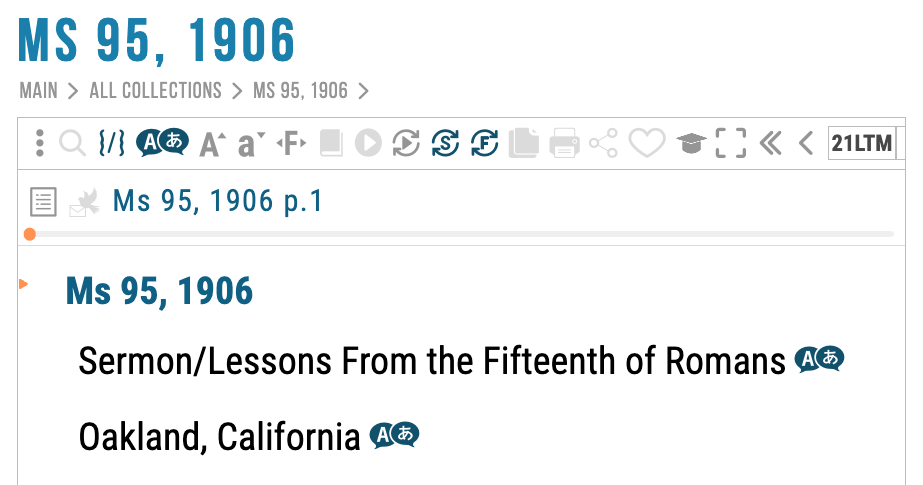
\includegraphics[width=1\linewidth]{images/sermons-and-talks.png}
    \label{fig:enter-label}
\end{figure}


\begin{figure}
    \centering
    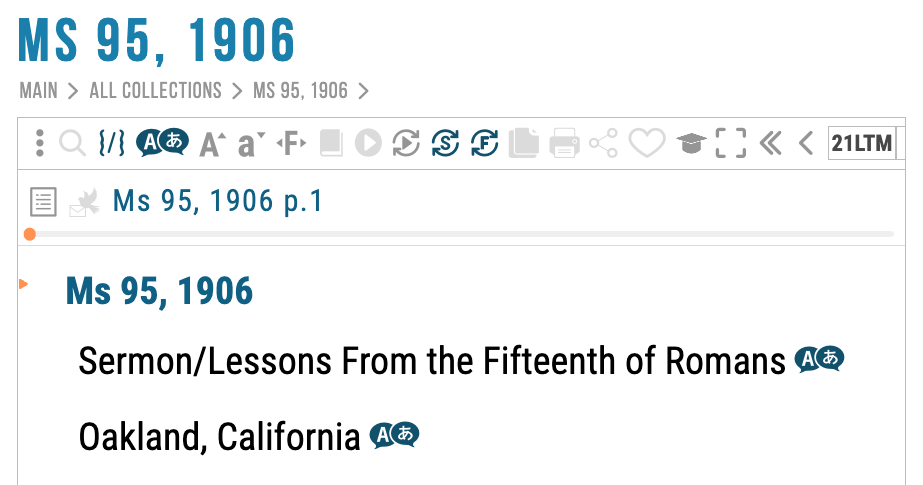
\includegraphics[width=1\linewidth]{images/sermons-and-talks.png}
    \label{fig:enter-label}
\end{figure}


For us, personally, these quotations are unauthenticated and, especially, invalid compared to Ellen White’s authenticated works. But if someone insists on weighing her unconfirmed reports and published writings equally, we will not stand in their way but even further push the conclusion of the Holy Spirit as a being. Let’s follow together.


Dla nas osobiście te cytaty są nieuwierzytelnione i, szczególnie, nieważne w porównaniu z uwierzytelnionymi dziełami Ellen White. Ale jeśli ktoś nalega na równe traktowanie jej niepotwierdzonych doniesień i opublikowanych pism, nie będziemy temu przeciwni, ale jeszcze bardziej podkreślimy wniosek o Duchu Świętym jako istocie. Podążajmy razem.


Even compared with Ellen White’s authenticated works, such a Holy Spirit, a being, would not be one with God because Christ was \egwinline{\textbf{The only being who was one with God}}[Lt121-1897.7; 1897][https://egwwritings.org/?ref=en\_Lt121-1897.7&para=7266.13]. This Holy Spirit, a being, could not \egwinline{\textbf{enter into all the counsels and purposes of God}}, because Christ was \egwinline{\textbf{the only being}}[PP 34.1; 1890][https://egwwritings.org/?ref=en\_PP.34.1&para=84.75] who could do that. This Being is not to be exalted because \egwinline{\textbf{The Father and the Son \underline{alone} are to be exalted}}[YI, July 7, 1898 par.2.; 1898][https://egwwritings.org/?ref=en\_YI.July.7.1898.par.2&para=469.2964]. The Holy Spirit, as a being, would not fit in the order of heaven as the third being because Satan was \egwinline{\textbf{next to Christ the most exalted \underline{being}} in the heavenly courts}[RH August 9, 1898, par. 7; 1898][https://egwwritings.org/?ref=en\_RH.August.9.1898.par.7&para=821.17145]. This Holy Spirit, a being, was not invested in the cost of salvation; neither was he in the covenant with Father and Son to save the world, nor dishonored by man’s transgression.


Nawet w porównaniu z uwierzytelnionymi dziełami Ellen White, taki Duch Święty, istota, nie byłby jednością z Bogiem, ponieważ Chrystus był \egwinline{\textbf{Jedyną istotą, która była jednością z Bogiem}}[Lt121-1897.7; 1897][https://egwwritings.org/?ref=en\_Lt121-1897.7&para=7266.13]. Ten Duch Święty, istota, nie mógłby \egwinline{\textbf{wejść we wszystkie rady i zamiary Boga}}, ponieważ Chrystus był \egwinline{\textbf{jedyną istotą}}[PP 34.1; 1890][https://egwwritings.org/?ref=en\_PP.34.1&para=84.75], która mogła to zrobić. Ta Istota nie ma być wywyższana, ponieważ \egwinline{\textbf{Ojciec i Syn \underline{jedynie} mają być wywyższeni}}[YI, July 7, 1898 par.2.; 1898][https://egwwritings.org/?ref=en\_YI.July.7.1898.par.2&para=469.2964]. Duch Święty, jako istota, nie pasowałby do porządku nieba jako trzecia istota, ponieważ Szatan był \egwinline{\textbf{zaraz po Chrystusie najbardziej wywyższoną \underline{istotą}} w niebiańskich dworach}[RH August 9, 1898, par. 7; 1898][https://egwwritings.org/?ref=en\_RH.August.9.1898.par.7&para=821.17145]. Ten Duch Święty, istota, nie był zaangażowany w koszt zbawienia; nie był też w przymierzu z Ojcem i Synem, aby zbawić świat, ani nie został znieważony przez występek człowieka.


\egwinline{The great gift of salvation has been placed within our reach at an \textbf{infinite cost to the Father and the Son}.}[RH November 21, 1912, par. 2; 1912][https://egwwritings.org/?ref=en\_RH.November.21.1912.par.2&para=821.33329]


\egwinline{Wielki dar zbawienia został umieszczony w naszym zasięgu za \textbf{nieskończony koszt dla Ojca i Syna}.}[RH November 21, 1912, par. 2; 1912][https://egwwritings.org/?ref=en\_RH.November.21.1912.par.2&para=821.33329]


\egwinline{In the plan to save a lost world, the counsel was between them \textbf{\underline{both}}; \textbf{the covenant of peace was between the Father and the Son}.}[ST December 23, 1897, par. 2; 1897][https://egwwritings.org/?ref=en\_ST.December.23.1897.par.2&para=820.14803]


\egwinline{W planie ratowania zgubionego świata, narada była między nimi \textbf{\underline{oboma}}; \textbf{przymierze pokoju było między Ojcem a Synem}.}[ST December 23, 1897, par. 2; 1897][https://egwwritings.org/?ref=en\_ST.December.23.1897.par.2&para=820.14803]


\egwinline{But in the transgression of man \textbf{\underline{both} the Father and the Son were dishonored}.}[ST December 12, 1895, par. 7; 1895][https://egwwritings.org/?ref=en\_ST.December.12.1895.par.7&para=820.13243]


\egwinline{Ale w przestępstwie człowieka \textbf{\underline{zarówno} Ojciec, jak i Syn zostali znieważeni}.}[ST December 12, 1895, par. 7; 1895][https://egwwritings.org/?ref=en\_ST.December.12.1895.par.7&para=820.13243]


Such a Holy Spirit, a being, does not fit into harmony with the authenticated reports of Ellen White, nor with the Scriptures. The Holy Spirit is called ‘\textit{spirit}’, so it is a spirit, exclusively.


Taki Duch Święty, jako istota, nie jest zgodny z uwierzytelnionymi relacjami Ellen White, ani z Pismem Świętym. Duch Święty jest nazywany ‘\textit{duchem}’, więc jest duchem, wyłącznie.


Many of Sister White’s quotations are sourced from sermons or talks that were published after her death. In what follows, we will present a few that are most often discussed in an effort to prove that Sister White was a trinitarian. We invite everyone to weigh these quotations with her authenticated and published work, those during her lifetime.


Wiele cytatów Siostry White pochodzi z kazań lub przemówień, które zostały opublikowane po jej śmierci. W dalszej części przedstawimy kilka, które są najczęściej omawiane w celu udowodnienia, że Siostra White była trynitarianką. Zapraszamy wszystkich do porównania tych cytatów z jej uwierzytelnionymi i opublikowanymi dziełami, tymi za jej życia.


“\textit{And then the golden harps are touched, and the music flows all through the heavenly host, and they fall down and worship the Father and the Son and the Holy Spirit}.”\footnote{\href{https://egwwritings.org/?ref=en_Ms139-1906.32&para=9579.38}{EGW; Ms139-1906.32; 1906}} [Sermon/Thoughts on Matthew 4. Oakland, California July 24, 1906; Previously unpublished.]


“\textit{A potem złote harfy są dotykane, a muzyka płynie przez wszystkie zastępy niebiańskie, i padają oni, oddając pokłon Ojcu i Synowi, i Duchowi Świętemu}.”\footnote{\href{https://egwwritings.org/?ref=en_Ms139-1906.32&para=9579.38}{EGW; Ms139-1906.32; 1906}} [Kazanie/Rozważania na temat Mateusza 4. Oakland, Kalifornia 24 lipca 1906; Wcześniej niepublikowane.]


“\textit{We need to realize that the Holy Spirit, who is as much a person as God is a person, is walking through these grounds.}”\footnote{\href{https://egwwritings.org/?ref=en_Ms66-1899.11&para=6622.19}{EGW; Ms66-1899.11: 1899}} [Talk/Extracts From Talks Given by Mrs. E. G. White at the Opening of College Hall, Avondale, and in the Avondale Church]


“\textit{Musimy zdać sobie sprawę, że Duch Święty, który jest tak samo osobą, jak Bóg jest osobą, przechadza się po tych terenach.}”\footnote{\href{https://egwwritings.org/?ref=en_Ms66-1899.11&para=6622.19}{EGW; Ms66-1899.11: 1899}} [Przemówienie/Fragmenty przemówień wygłoszonych przez panią E. G. White podczas otwarcia College Hall, Avondale, oraz w kościele Avondale]
